\section{Implementation and Evaluation}
\label{sec:implementation}

\begin{figure*}[ht]
  \centering
  \makebox[\linewidth][c]{%
  \begin{subfigure}[b]{0.5\linewidth}
    \includegraphics[width=\linewidth]{neighbour-fixed/throughput-vs-population}
    \caption{Every node make transactions with a fixed node.}
    \label{fig:global-throughput-fixed}
  \end{subfigure}%
  \begin{subfigure}[b]{0.5\linewidth}
    \includegraphics[width=\linewidth]{neighbour-random/throughput-vs-population}
    \caption{Every node make transactions with a random node.}
    \label{fig:global-throughput-random}
  \end{subfigure}
  }
  \caption{Global throughput increases as the population increases when every node transact at the same rate.
  Making transactions with fixed nodes results in a higher throughput because of the caching mechanism.}
  \label{fig:global-throughput}
\end{figure*}

A free and open source implementation can be found on GitHub: \url{https://github.com/kc1212/checo}.
It implements the three protocols and the Extended TrustChain.
We also implement the caching optimisation discussed in \Cref{sec:caching}.
It is written in the Python programming language.
The cryptography primitives we use are SHA256 for hash functions and Ed25519 for digital signatures.

We run the experiment on the DAS-5\footnote{\url{https://www.cs.vu.nl/das5/}} with up to 1200 nodes.
Every node makes transactions at 2 per second.
Since Bitcoin transactions are approximately 500 bytes~\cite{txsize},
we use a uniformly random transaction size sampled between 400 and 600 bytes.

The global throughput results are shown in~\Cref{fig:global-throughput}.
We consider~\Cref{fig:global-throughput-fixed} as the ideal case,
where nodes only make transactions with a fixed node.
\Cref{fig:global-throughput-random} is the worst case,
where nodes make transactions with random nodes and the caching mechanism is unlikely to be used.
Observe that the transaction rate is much lower in~\Cref{fig:global-throughput-random},
which is because the communication of an agreed fragment is necessary to verify every transaction (no caching),
putting a strain on our network infrastructure.
% In practice, we do not expect such behaviour to occur as it is possible to cache agreed fragments.

For~\Cref{fig:global-throughput-fixed},
the magnitude of our throughput may not be self-evident at first glance.
Recall that we fixed the transaction rate to 2 TPS,
but how is it possible to have around 4800 transactions per second for 1200 nodes (which is 4 TPS)?
It is due to the way validated transactions are calculated.
Transactions are between two parties, hence if every node makes two transactions per second,
every node also expects to receive two transactions per second.
Hence, for every node, the TX blocks are created at 4 per second.
Validation requests are sent at the same rate, which explains the magnitude.
Overall, the throughput has a linear relationship with the population size.
This result is a strong indication of the horizontal scalability which we aimed to achieve.

The downside of our design is that the communication complexity of the consensus protocol grows polynomially as the number of facilitators grows linearly.
Hence, the consensus protocol will take longer to complete, and larger fragments must be sent for transaction verification.
On the other hand, it does not significantly impact the throughput;
only the transaction verification delay is affected.
We refer the reader to~\cite[Chapter 5]{checo} for additional analysis of the effect of the number of facilitators as well as other experimental results.

% The difference in magnitude between \Cref{fig:global-throughput-fixed} and \Cref{fig:global-throughput-random} is caused by the caching mechanism mentioned earlier.
% If a new agreed fragment needs to be transmitted to validate every transaction then it puts a toll on the network infrastructure.
% The low transaction rate in~\Cref{fig:global-throughput-random} is caused by the fact that the network infrastructure cannot keep up with our demand.
% In practice, we do not expect such behaviour to occur as it is possible to cache agreed fragments.
